\documentclass[tikz]{standalone}
\usepackage{pgfplots}
\pgfplotsset{compat=1.15}
\usepackage{mathrsfs}
\usetikzlibrary{arrows,calc}
\usepackage{tkz-euclide}

\usepackage{fp}
\pagestyle{empty}

\definecolor{AngleClr}{rgb}{0,0.39215686274509803,0}
\definecolor{ShapeClr}{rgb}{0.6,0.2,0}

\begin{document}

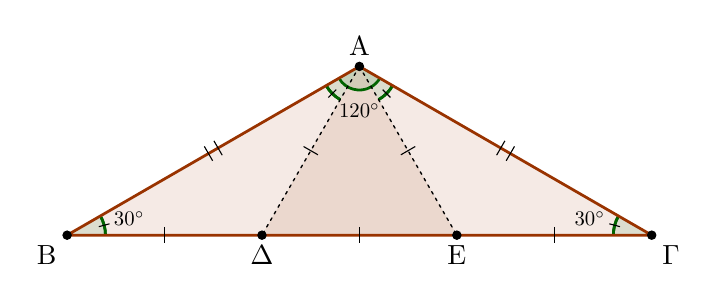
\begin{tikzpicture}[scale=.75]
\tkzSetUpLine[line width=1pt,color=black]
\tkzSetUpPoint[fill=black]

\def\Scale{1.1}
\FPeval{\Ax}{3 * \Scale}
\FPeval{\Ay}{0.866 * \Ax}
\FPeval{\Bx}{0.5 * \Ax}
\FPeval{\Cx}{1.5 * \Ax}

\tkzDefPoints{-\Cx/0/B,0/\Ay/A,\Cx/0/C,-\Bx/0/D,\Bx/0/E}


\tkzFillPolygon[fill=ShapeClr,fill opacity=0.1](A,B,C)
\tkzFillPolygon[fill=ShapeClr,fill opacity=0.1](A,D,E)

% Angles equal to 30 degrees.
\tkzFillAngles[fill=AngleClr,size=.65,fill opacity=0.1](C,B,A B,A,D A,C,B E,A,C)
\tkzMarkAngles[line width=1pt,size=.65,color=AngleClr](C,B,A B,A,D A,C,B E,A,C)
\tkzMarkAngles[mark=|,mksize=2,line width=1pt,size=.65,color=AngleClr](C,B,A B,A,D A,C,B E,A,C)

\tkzFillAngle[fill=AngleClr,size=.4,fill opacity=0.1](B,A,C)
\tkzMarkAngle[line width=1pt,color=AngleClr,size=.4](B,A,C)

\tkzDrawPolygon[color=ShapeClr](A,B,C)
\tkzDrawPoints[size=3](A,B,C,D,E)
\tkzLabelPoint[above](A){$\rm A$}
\tkzLabelPoint[below left](B){$\rm B$}
\tkzLabelPoint[below right](C){$\rm \Gamma$};
\tkzLabelPoint[below](D){$\rm \Delta$}
\tkzLabelPoint[below](E){$\rm E$}

\tkzMarkSegments[mark=||,size=3](A,B A,C)

\tkzLabelAngle[scale=0.75,pos=1.45](C,B,A){$30^\circ$}
\tkzLabelAngle[scale=0.75,pos=1.45](A,C,B){$30^\circ$}
\tkzLabelAngle[scale=0.75](B,A,C){$120^\circ$}

\tkzDrawSegments[line width=0.5pt,color=black,dashed,dash pattern=on 1pt off 1.75pt](A,D A,E)

\tkzMarkSegments[mark=|,size=3](A,E A,D D,E B,D E,C)

\end{tikzpicture}

\end{document}
